\newcommand{\pie}[1]{%
\begin{tikzpicture}
 \draw (0,0) circle (1ex);\fill (1ex,0) arc (0:#1:1ex) -- (0,0) -- cycle;
\end{tikzpicture}%
}

\newcommand{\revpie}{%
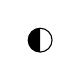
\begin{tikzpicture}
 \draw (0,0) circle (1ex);\fill (0,1ex) arc (90:270:1ex) -- (0,0) -- cycle;
\end{tikzpicture}%
}

\newcommand{\tableYes}{\pie{360}}
\newcommand{\tableNo}{\pie{0}}
\newcommand{\tablePartial}{\revpie}

\begin{table}[!t]
    \renewcommand{\arraystretch}{1.35}
    \newcolumntype{L}{>{\raggedleft\arraybackslash}X}
    \newcolumntype{C}{>{\centering\arraybackslash}X}
    \newcolumntype{R}{>{\raggedright\arraybackslash}X}
    \centering

    \begin{tabularx}{.9\linewidth}{l C C C}
        \toprule
                                           & AWS           & Azure         & GCP           \\
        \hline                                                              
        TEE                                & \tableYes     & \tablePartial & \tableYes     \\
        Firmware                           & \tableYes     & \tablePartial & \tablePartial \\
        Kernel                             & \tablePartial & \tablePartial & \tablePartial \\
        Root FS                            & \tablePartial & \tablePartial & \tablePartial \\
        \hline                                                              
        \textbf{Nominal AL}                & \textbf{4}    & \textbf{4}    & \textbf{4}    \\
        \textbf{Trustworthy AL}            & \textbf{2}    & \textbf{0}    & \textbf{1}    \\
        \bottomrule
    \end{tabularx}

        \vspace{0.2cm}
        {\raggedright \tableYes\xspace= Verifiable w/o trust; \tablePartial\xspace= Verifiable w/ trust; \tableNo\xspace= Not verifiable \par}
        \vspace{0.2cm}
        \caption{AMD \sevsnp{} offerings on \ac{AWS}, Azure and \ac{GCP}. This
          table reflects attestation levels described in
          \cref{section:att-levels} and verifiability with or
          without trust, resulting in the maximum nominal AL (with trust in the
          \ac{CSP}) and trustworthy AL (without trust). Results dated \clouddate.}
        \label{tbl:cloud-landscape}
        %\vspace{-5mm}
\end{table}
%
  
